\documentclass[14pt, a2paper, portrait,innermargin=5mm,
blockverticalspace=5mm, colspace=5mm, subcolspace=3mm]{tikzposter}
% font size: The size of the text in the main body may be set as : 12pt, 14pt, 17pt, 20pt, or 25pt;
% paper size: Currently, paper sizes may be set to : a0paper, a1paper, or a2paper;
% orientation: Either landscape or portrait
\usepackage[utf8]{inputenc}
\usepackage[T1]{fontenc}

\usepackage{rustic}
\usepackage{lmodern}
\usepackage[sfdefault,lf]{carlito}
\usepackage{fontawesome}
\usepackage{blindtext}
\usepackage{comment}
\usepackage{hyperref}


\usepackage{listings}

\usetheme{Simple}
%\usetitlestyle{Empty}\usebackgroundstyle{Empty}

%--------------------------------------
%-------------- FARBEN

\usepackage[usenames, dvipsnames]{color} % um diese Color-Names zu verwenden: https://de.sharelatex.com/learn/Using_colours_in_LaTeX#!#Reference_guide z.B. \color{RubineRed}

\definecolor{GrafRed}{RGB}{102,0,34} %#660022
\definecolor{GrafBeige}{RGB}{226,212,186}

\definecolor{LightGrafRed}{RGB}{152,51,85} %#A3244E

%---------------- bei den Farben gibt es immer bg und fg, wobei bg Hintergrund und fg normalerweise Schriftfarbe ist. Dies ist zu definieren für backgroundcolor, framecolor, dann für titlefg/bgcolor, selbiges für (inner)blocktitle und blockbody, und ggf. für notefg/bgcolor
\colorlet{titlebgcolor}{GrafRed}
\colorlet{titlefgcolor}{GrafBeige}
\colorlet{blocktitlefgcolor}{GrafRed}

%---------------------- Code-Bsps
\definecolor{Text}{RGB}{0.36, 0.54, 0.66}
\definecolor{Element}{RGB}{0.53, 0.66, 0.42}
\definecolor{Attr}{RGB}{0.6, 0.4, 0.8}

\lstdefinelanguage{XML}
{
  morestring=[b]",
  morestring=[s]{>}{<},
  morecomment=[s]{<!--}{-->},
  morekeywords={xmlns,version,type,canonicalRef,metr,real,target}% list your attributes here
}

\lstset{language=XML,
showspaces=false,
showtabs=false,
basicstyle=\ttfamily,
columns=fullflexible,
breaklines=true,
showstringspaces=false,
breakatwhitespace=true,
escapeinside={(*@}{@*)},
basicstyle=\ttfamily\footnotesize,
stringstyle=\color{Text},
commentstyle=\color{Element}\upshape,
keywordstyle=\color{SpringGreen}\bfseries,
}


%---------------------------- Title-Infos und Package-Wirrwarr

\title{{\rustfamily\bfseries Grazer Repositorium antiker Fabeln}}
%\author{Prof. Dr. Ursula Gärtner, Sarah Lang}
%\date{\today}
\author{Institut für Klassische Philologie \& Zentrum für Informationsmodellierung, Karl-Franzens-Universität Graz}
%\institute{Institute of Classics, Karl-Franzens-Universität Graz}
\titlegraphic{\hspace{2cm}
\includegraphics[height=7.5cm, right]{graf-logo-beige.png}}

%----------------------------------------------------------------------
% Title definieren
\definetitlestyle{sampletitle}{
width=\paperwidth, linewidth=2pt, innersep=5pt,
titletotopverticalspace=0mm, titletoblockverticalspace=10mm
}{
\begin{scope}[line width=\titlelinewidth]
\draw[color=blocktitlebgcolor, fill=titlebgcolor]
(\titleposleft,\titleposbottom) rectangle (\titleposright,\titlepostop);
\end{scope}
}
%---------------------- und so weiter... geht alles nicht..
\settitle{\begin{tabular*}{0.8\textwidth}{r p{0.7\textwidth}}%
\@titlegraphic & \vbox{%
\centering%
\color{titlefgcolor} {\bfseries \Huge \sc \@title \par}
\vspace*{1em}
{\huge \@author \par} \vspace*{0.5em} {\LARGE \@institute}
} \end{tabular*}
}

\usetitlestyle{sampletitle}


%line-overflow meiden, dazu hinter begin{doc} \sloppy
\setlength{\emergencystretch}{2pt}

 %--------------------- PDF-Info
 \hypersetup{
    pdftitle={GRaF},
    pdfauthor={Sarah Lang},
    pdfsubject={GRaF project},
    pdfkeywords={GRaF; GAMS repository; ancient fables},
    colorlinks=false,           % no link border color
    pdfa,
}


 
 %--------------------------------------
 % new commands für CV-Icons
 
 % 1. Argument=favicon; 2. Argument=Text; 3.+4.=ColorName; 5.Schriftgröße z.B. \Large
 
 % cvicon command
 \newcommand{\cvicon}[4]{%
\vspace{0.5pt}\begin{minipage}[t]{0.12\textwidth}\vspace{0pt}%
 \begin{tabular*}{0.125\textwidth}{c c}%
{\color{#3}\centering\Large #1} & \phantom{}\\%  
{\color{#4}\footnotesize\sffamily \parbox[t]{\textwidth}{\centering#2}} & \phantom{}\\%
\end{tabular*} \end{minipage} \hfill%
  }
 
  % bigicon command
 \newcommand{\bigicon}[4]{%
\vspace{0.5pt}\begin{minipage}[t]{0.12\textwidth}\vspace{0pt}%
 \begin{tabular*}{0.125\textwidth}{c c}%
{\color{#3}\centering\Huge #1} & \phantom{}\\%  
{\color{#4}\Large\sffamily \parbox[t]{\textwidth}{\centering#2}} & \phantom{}\\%
\end{tabular*} \end{minipage} \hfill%
  }

  % bullettpoint command
 \newcommand{\bullettpoint}[5]{%
\vspace{0.35em}\begin{minipage}[t]{\textwidth}\vspace{0pt}%
 \begin{tabular*}{0.125\textwidth}{c c}%
{\color{#3}\centering#5 #1\phantom{}} & {\color{#4}#5\sffamily \parbox[t]{\textwidth}{#2}}\\%  
\end{tabular*}\vspace{0.15em} \end{minipage}\hfill%
  }
%----------------------------------------------------------------




\begin{document}

\maketitle

\block{{\rustfamily\bfseries Das Projekt: Fabula docet -- Wer will schon saure Trauben}?}
{

Das \textbf{``Grazer Repositorium antiker Fabeln'' (GRaF)} ist ein \textbf{Sparkling Science Projekt}, das unter aktiver Beteiligung von Schulklassen eine \textbf{wissenschaftliche Schulausgabe antiker Fabeln} (textkritischer Apparat, Vokabelangaben, Übersetzung, Sacherklärungen und Paralleltexten) erarbeitet, die als \textbf{digitale Edition in TEI-XML} auf dem \textbf{Grazer GAMS-Repository} als digitale Repräsentation verfügbar gemacht wird:Es handelt sich bei GRaF um ein \textbf{wissenschaftliches Webportal zu antiken Fabeln}, das \textbf{auch eine ``digitale Schulausgabe'' anbietet}, die als \textbf{dynamische Repräsentation aus langzeitarchivierten Daten} generiert wird. GRaf versteht sich \textbf{nicht als ``Lernplattform''}, sondern als innovativen Ansatz, der die \textbf{Prinzipien einer kommentierten und annotierten wissenschaftlichen Digitalen Edition in TEI-XML} mit dem \textbf{neuen Konzept des ``Digitalen Schulbuchs''} verbindet.
Die Basisdaten werden von den am Projekt beteiligten \textbf{Schulklassen unter wissenschaftlicher Anleitung erarbeitet} und \textbf{durch wissenschaftliche Einführungen, eine Phaedrus-Bibliographie und ein wissenschaftliches Netzwerk zur Fabelforschung angereichert.} 
Damit schlägt sie den Bogen zwischen \textbf{Wissenschaft und Citizen Science} und ermöglicht den Schülern, Einblick in einen literaturwissenschaftlichen Umgang mit Fabeln zu erlangen. Die Ergebnisse des Sparkling Science-Projekts werden außerdem fachdidaktisch ausgewertet.



\vspace{1.5em}

\bigskip

%------------ das hier ginge auch mit dem nicht TikzPoster-eigenen \colorbox{GrafRed}{Inhalt}, schaut aber nicht ganz so schön aus und passt sich nicht von allein an die Poster-Box an..

\coloredbox[roundedcorners,bgcolor=GrafRed,fgcolor=GrafBeige,framecolor=GrafRed]{
      \Huge\begin{minipage}[c]{0.95\textwidth} % Start the right-hand side of the page
      \bigskip
\bigicon{\faUsers}{Schule}{GrafBeige}{GrafBeige}
\bigicon{\faLaptop}{Webportal}{GrafBeige}{GrafBeige}
\bigicon{\faUniversity}{Citizen Science}{GrafBeige}{GrafBeige}
\bigicon{\faKeyboardO}{{\large Digital Humanities}}{GrafBeige}{GrafBeige}
\bigicon{\faGraduationCap}{Universität}{GrafBeige}{GrafBeige} \phantom{  }

\end{minipage}
}

\bigskip



    \normalsize
}


  \begin{columns}    
    \column{0.35}
    \block{{\rustfamily Kooperationspartner}}{
\hspace{1em}
\begin{minipage}[t]{0.28\textwidth}\vspace{0pt}


\bigskip

{\small

{\bfseries International} \\
\bullettpoint{\faUser}{PD Dr. Nicola Hömke}{}{}{}
\bullettpoint{\faUser}{Dr. Alexandra Forst}{}{}{}
\bullettpoint{\faUser}{Peggy Klausnitzer}{}{}{}
\bullettpoint{\faUniversity}{Klassische Philologie, Universität Potsdam}{}{}{}

\bigskip
\vspace{1em}

{\bfseries Beteiligte Schulen} \\
\bullettpoint{\faUniversity}{Akademisches Gymnasium, Graz}{}{}{}
\bullettpoint{\faUniversity}{BRG Petersgasse, Graz}{}{}{}
\bullettpoint{\faUniversity}{BG Rein, Gratwein-Straßengel}{}{}{}
\bullettpoint{\faUniversity}{Lise-Meitner-Gymnasium, Falkensee (DE)}{}{}{}

\bigskip
}

\end{minipage}\hfill

\bigskip

  }

    \column{0.33}
    \block{}{
        
\begin{minipage}[t]{0.3\textwidth}\vspace{0pt}

\bigskip
\coloredbox[width=0.9\textwidth,bgcolor=GrafBeige,fgcolor=GrafRed,framecolor=GrafBeige]{



\bullettpoint{\faMousePointer}{wissenschaftliches Webportal}{}{}{}\\
\bullettpoint{\faMousePointer}{`digitale Schulausgabe'}{}{}{}\\
\bullettpoint{\faMousePointer}{langzeitarchivierte Basisdaten}{}{}{}\\

\bigskip

\begin{tikzfigure}
            \includegraphics[width=0.75\textwidth]{fabelbuch.jpg}
        \end{tikzfigure}
        
        \bigskip

}
 \end{minipage}\hfill
        
    }  

    \column{0.33}
    \block{{\rustfamily Zusatz-Features}}{
        \begin{enumerate}
            \item Grazer Latein Tage
            \item Grazer Fabelnetzwerk: \\ \protect\url{grafnetzwerk.wordpress.com}
            \item Phaedrus-Bibliographie
            \item wissenschaftliche Einführungen
            \item dynamisch generierte Arbeitsblätter für Lehrende
        \end{enumerate}
    }
    
    
    \faUsers
    \faUniversity
    \faBook
    \faGraduationCap
    \faDocumentO
\end{columns}


\begin{columns}
   \column{0.36}
    \block{}{
    \coloredbox[width=0.3\textwidth,roundedcorners,bgcolor=GrafBeige,fgcolor=GrafBeige,framecolor=GrafBeige]{
        \begin{tikzfigure}
            
\includegraphics[width=0.07\textwidth]{zim_rot.png}
            
\includegraphics[width=0.07\textwidth]{kfFarbe.jpg}\hspace{0.5em}
            
\includegraphics[width=0.07\textwidth]{graf-logo-rot.png}
            
            \vspace{1em}
            \bigskip


\includegraphics[width=0.07\textwidth]{oead-transp.png}\hspace{0.5em}

\includegraphics[width=0.07\textwidth]{bmwfw-transp.png}\hspace{0.5em}

\includegraphics[width=0.07\textwidth]{gamslogo.png}

\vspace{1em}
            \bigskip
            
\includegraphics[width=0.23\textwidth]{sparklingScience.jpg}
            
            \bigskip\phantom{}
        \end{tikzfigure}
         }
    }
    
    \column{0.27}
    \block{{\rustfamily Kontakt}}{
      \begin{minipage}[t]{0.25\textwidth}\vspace{0pt}
\bullettpoint{\faUniversity}{Institut für Klassische Philologie}{}{}{}
\bullettpoint{\faMapMarker\phantom{}}{Universitätsplatz 3/II, 8010 Graz}{}{}{}
\bullettpoint{\faPhone}{Tel: +43 (0)316 380 -- 2430}{}{}{}
\bullettpoint{\faAt}{\protect\url{klassphil@uni-graz.at}}{}{}{}

    \bullettpoint{\faRefresh}{Mitmachen!}{}{}{\Large}\\
    
   \vspace{1em}     
%\bullettpoint{\faMousePointer}{\url{https://gams.uni-graz.at/graf}}{}{}{}\\
\bullettpoint{\faClockO}{\textbf{Laufzeit:} 01.10.2017--30.09.2019}{}{}{}\\
\bullettpoint{\faClipboard}{\textbf{Projektleitung:} Dr. Ursula Gärtner}{}{}{}\\
    
    \end{minipage}\hfill
    }
    \column{0.32}
    \block{}
    {
    \coloredbox[width=0.29\textwidth,roundedcorners,bgcolor=GrafRed,fgcolor=GrafRed,framecolor=GrafRed]{
    \begin{tikzfigure}
            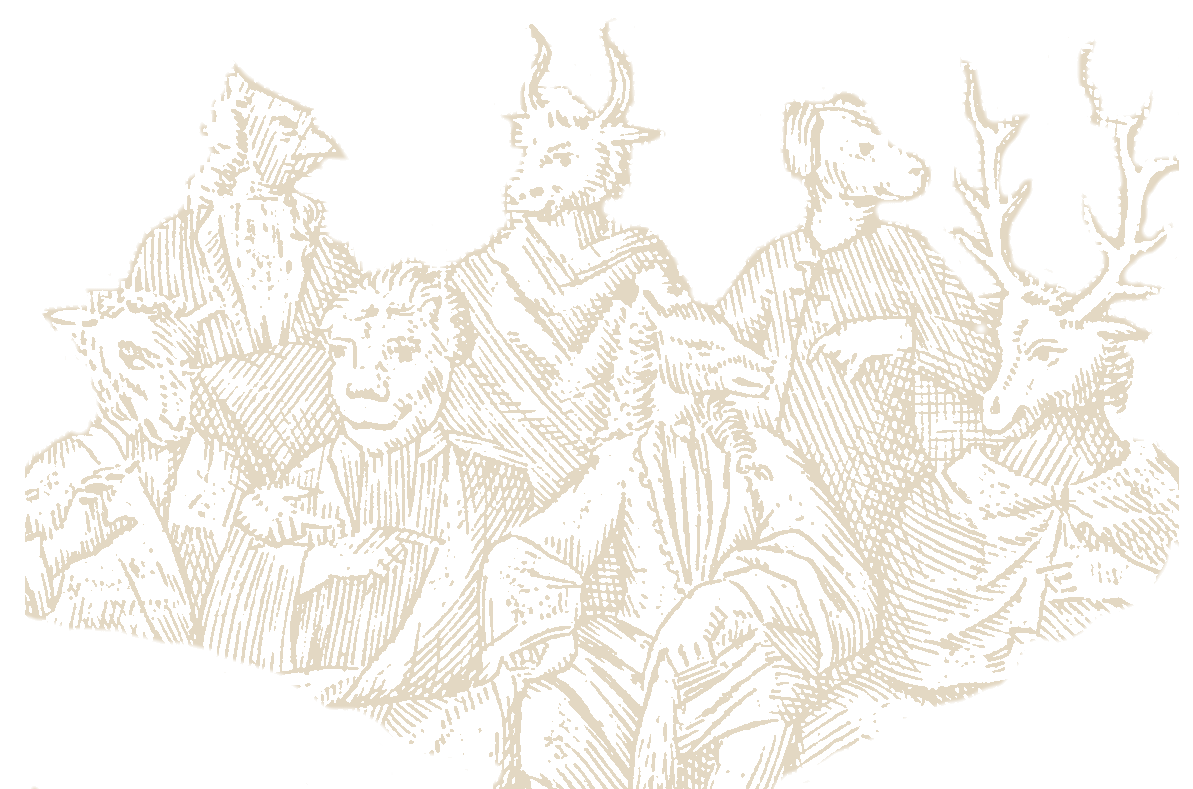
\includegraphics[width=0.23\textwidth]{tiere-transparent-beige.png}
        \end{tikzfigure}
        \phantom{ }
       } 
       
       \bigskip
      
      \coloredbox[width=0.29\textwidth,roundedcorners,bgcolor=GrafBeige,fgcolor=GrafRed,framecolor=GrafBeige]{
     \begin{minipage}[t]{0.18\textwidth}\vspace{0pt}  
      
   \small
   \protect\url{https://gams.uni-graz.at/graf}
      \phantom{}
      \end{minipage}\hfill
      \begin{minipage}[t]{0.08\textwidth}\vspace{0pt}
   
\includegraphics[width=0.8\textwidth]{QR2035.jpg}
          \phantom{ }
          
          \end{minipage}\hfill
       } 
      
    }
    
\end{columns}

\end{document}
